\documentclass[]{article}

\usepackage{algorithm}
\usepackage[noend]{algpseudocode}
\usepackage{cite}
\usepackage{graphicx}
\usepackage{xcolor}

% Use commented out command when done
%\newcommand{\comment}[1]{}
\newcommand{\comment}[1]
{\par {\bfseries \color{green} #1 \par}}

%opening
\title{Haiku Generations}
\author{Zachary A Bookey \and Max Magnuson}

\begin{document}

\maketitle

\begin{abstract}
Something something I'm really bad at abstracts...
\end{abstract}

\section{Introduction}
Give a quick overview of what we did for our project.

\section{Background}

\subsection{Haiku}
Haikus are three line poems with the second line longer than the other two. In english haikus the lines are measured by the number of syllables. The most common configuration is 5-7-5 in which the first and second lines of the poem have five syllables, and the second line of the poem has seven syllables. Figure \ref{fig:WrightHaiku} uses this structure. Some haikus contain fewer than seventeen syllables, but rarely exceed that amount \cite{Higginson}. \comment{"Need to explain syllables?"}

\begin{figure}[H]
	\centering
	From the skyscraper, \break
	All the bustling streets converge \break
	Towards a spring sea.
	\caption{Haiku composed by Richard Wright \cite{Terebess}}
	\label{fig:WrightHaiku}
\end{figure}

Due to the constraints of haikus, authors need to be careful in choosing each word. With so few syllables to work with, each word contributes significantly more to the overall meaning of the poem than other poetic forms. Therefore, haikus need to be terse and not use complete sentences. In figure \ref{fig:WrightHaiku} only the second line can be considered a complete sentence.

\subsection{Markov Chains}

Markov chains are a collection of states or variables with an associated collection of probabilities for each state that denotes the chance of going from one state to another. Markov chains can be represented as graphs. In figure \ref{fig:Chain} A, B, and C are nodes that represent the collection of states. The edges represent probabilities. For example, the likeliness of going from state A to state B is 0.25. Note that the edges of each node sum to 1. This is important to maintain because the nonzero edges connect to all possible states that can be achieved from a specific node. This means that in figure \ref{fig:Chain}, if the current state is B, then the possible states that follow are A and C. B cannot follow another B since the probability to itself is zero. \cite{Markov}

\begin{figure}[H]
	\centering
	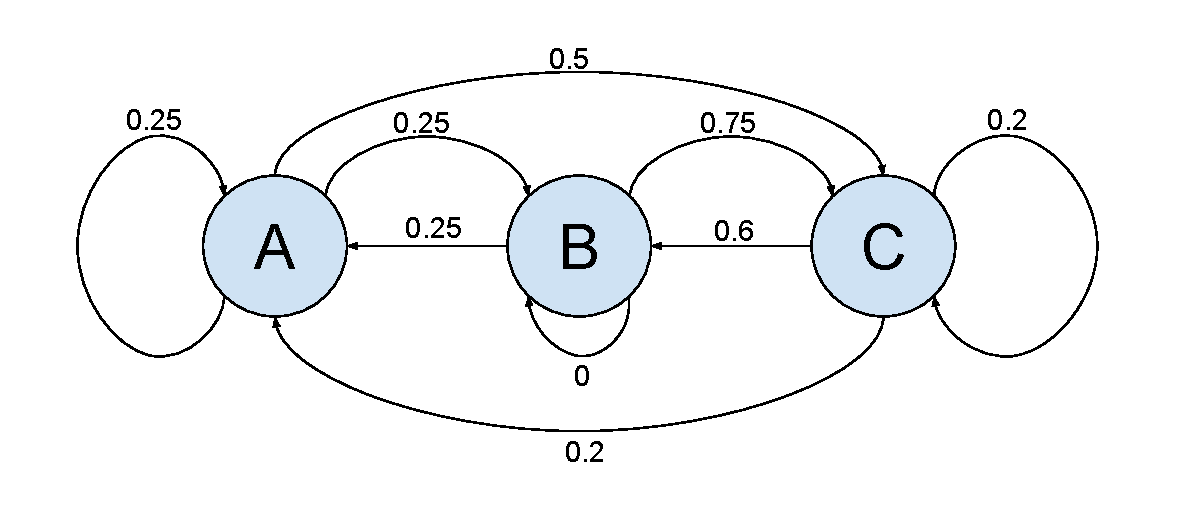
\includegraphics[width=1\textwidth]{MarkovChainExample}
	\caption{Example Markov Chain}
	\label{fig:Chain}
\end{figure}

\section{Haiku Constraints}
Demonstrate how a haiku can be represented as a constraint problem. For example explain how each word can be represented as a node and a link of nodes with the right number of syllables is a line and three lines makes a haiku.

\section{The Search Space}
Explain the basic concept of a markov chain and illustrate how we used it as our search space. Secondly describe how we parsed files in order to create this chain from lists of sentences/words.

\section{Search Algorithms}
Go over each search algorithm we implemented in detail.
\subsection{Naive Search}

\subsection{Short Random Walk}

\subsection{Depth First Search}
One of the methods we used to navigate the search space and generate a Haiku was depth first search with restarts. To accomplish this we utilized a two-way linked list where each node contained a markov node and generated it's child randomly by weighting each of the markov nodes children's probability to generate each line individually. To initialize the search we chose a random markov node from our markov chain and had our root list node point to this node. The algorithm then chose a child node from that markov node and determined how many syllables the line of words would currently have and if we're still within the constraint it would repeat. If we have exactly the number of syllables we needed the code would return the line represented by this linked list starting from the root and ending at the child. If the child we chose would violate our constraints we retreated to the parent and would randomly choose a child that we had not yet visited from this node. If no children we're available we would retreat up another node. Finally if we are at the root node and there are no children available the code would restart and choose a new random starting position in the markov chain.

\begin{algorithm}[H]
	\caption{$Depth\_First\_Search(n)$} \label{DFSB}
	\begin{algorithmic}[1]
		\State Choose an random $root$ node from the chain.
		\State $current = root$
		\While {$Syllables \neq n$}
			\If{Have not visited all possible children of $current$}
				\State Choose random unvisited $child$ of $current$
				\If{$child.syllables \leq n$}
					\State $current = child$
				\EndIf
			\Else
				\If{$current == root$}
					\Return $Depth\_First\_Search(n)$
				\Else
					\State $current$ = $parent$ of $current$
				\EndIf
			\EndIf
		\EndWhile
		\Return Line represented by linked list defined by $root$
	\end{algorithmic}
\end{algorithm}

This approach was then extended to try and maintain fluidity between lines. Instead of generating a random node for the starting position of the line we attempted to use a child of the last node from the previous line. If the child we chose was unable to produce a valid line for the haiku we chose a different child of the previous line's last node. If we had exhausted all the children then the algorithm opted to lose fluidity and generate a random starting node for this line.

\begin{algorithm}[H]
	\caption{$Depth\_First\_Search(node, n)$} \label{DFSB_WithStart}
	\begin{algorithmic}[1]
		\State $root = node$
		\State $current = root$
		\While {$Syllables \neq n$}
		\If{Have not visited all possible children of $current$}
		\State Choose random unvisited $child$ of $current$
		\If{$child.syllables \leq n$}
		\State $current = child$
		\EndIf
		\Else
		\If{$current == root$}
			\State {generate new $child$ from the $parent$ of $root$}
			\Return {$Depth\_First\_Search(child, n)$}
		\Else
		\State $current$ = $parent$ of $current$
		\EndIf
		\EndIf
		\EndWhile
		\Return Line represented by linked list defined by $root$
	\end{algorithmic}
\end{algorithm}

A final extension of this approach that is currently being implemented is to choose a starting node for the whole haiku and generate the entire haiku using just that node. Some haiku's generated by the previous approach would be valid in this sense but since any line could be restarted with random node not all haiku's would be fluid throughout. This approach would need to be able to regenerate the previous line if the children of the last node cannot generate a new line.

% Create pseudo code for this approach...

\section{Results}
Give some examples of the haiku's we were able to identify and acknowledge some of the highlights and short comings of the work we did.

\section{Conclusion}
Conclude yo.

\section{Related Work}
List of related works?

\bibliography{mybib}
\bibliographystyle{plain}
\end{document}
